\documentclass{beamer}
\author{Julius Elinson}
\usetheme{Frankfurt}
\usecolortheme{beaver}
\usepackage{multicol, amsmath,mathpazo}

\titlegraphic{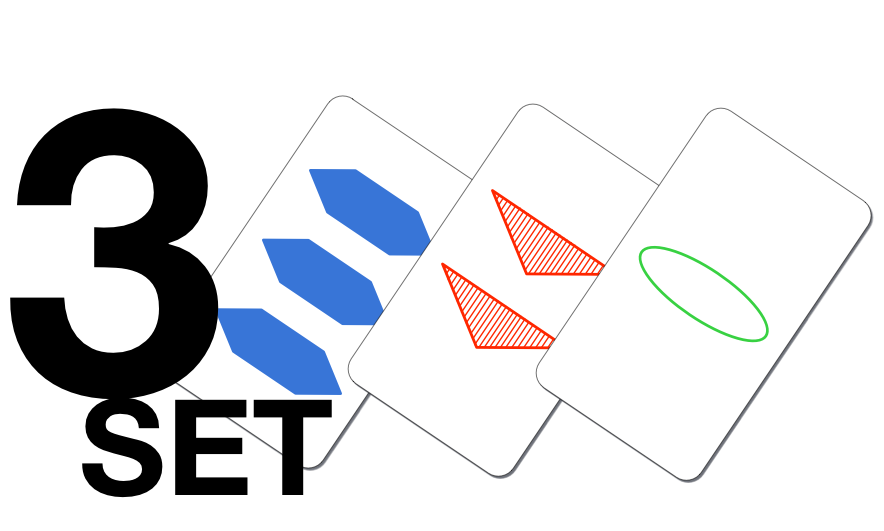
\includegraphics[width=.35\paperwidth]{img/logo.png}}

\title{3Set}
\subtitle{An iOS Game Of Mixing \& Matching}
\institute{Aquincum Institute of Technology\\Harvey Mudd College}
\logo{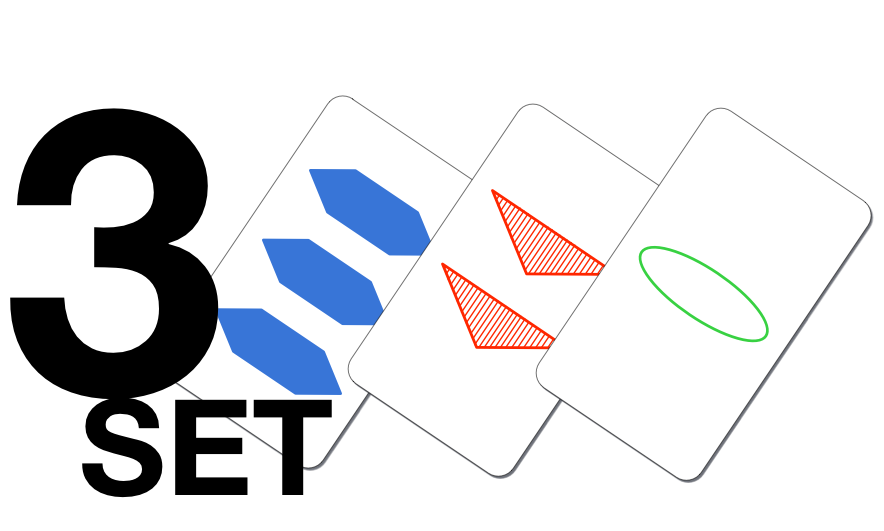
\includegraphics[width=.1\paperwidth]{img/logo.png}}

\beamertemplatenavigationsymbolsempty

\begin{document}
{
\setbeamertemplate{logo}{}
\begin{frame}
\maketitle
\end{frame}
}


\section{The Game}
\begin{frame}[t]{Set}

\textbf{Gameplay}:
\begin{itemize}
 \item A deck of 81 cards
 \item Each card has 4 attributes
 \item Each attribute has 3 possible values
\end{itemize}
\pause


\begin{figure}
\centering 
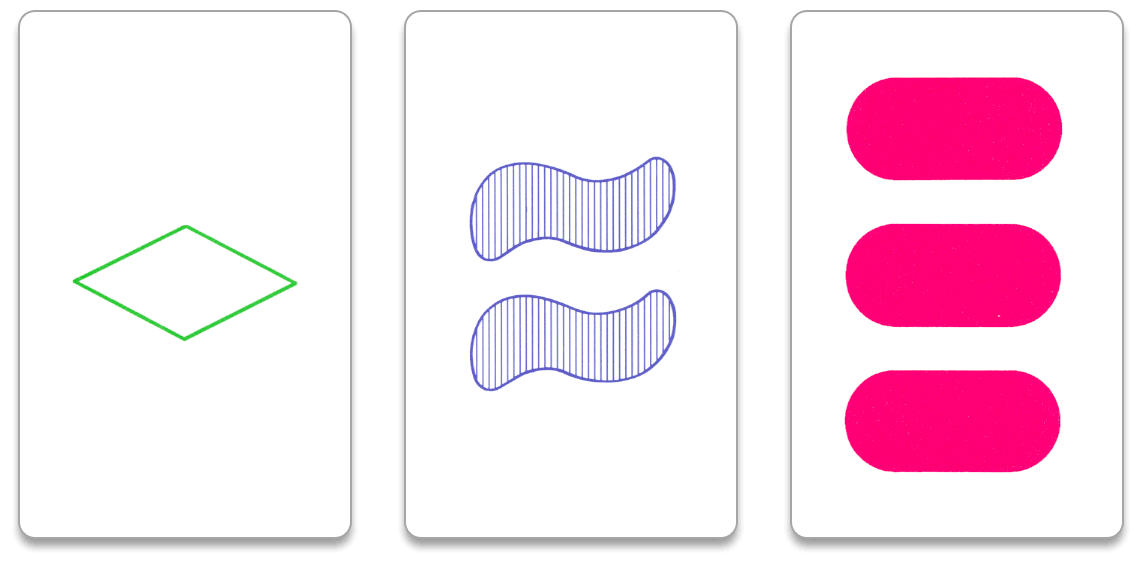
\includegraphics[width=.5\paperwidth]{img/triplet.png}
\end{figure}
\end{frame}

\begin{frame}[t]{Set}

\textbf{Goal}:
\begin{itemize}
 \item Create a \emph{set} of 3 cards, such that for each attribute, the values are either all the same or all different.
 \item<3-> There are about 12 cards shown at given time.
 \item<3-> Any number of players.
\end{itemize}

\begin{figure}
\centering 
\visible<2->{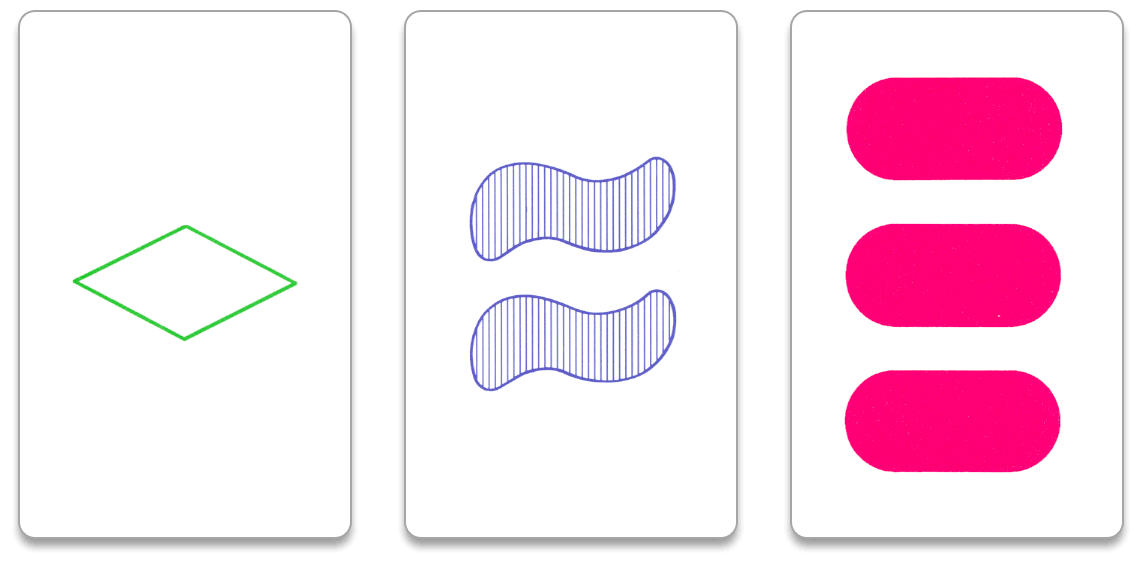
\includegraphics[width=.5\paperwidth]{img/triplet.png}}
\end{figure}

\end{frame}

\begin{frame}[t]{Set As An App}
\begin{itemize}
\pause
 \item The official app -- only for iPad
 \item Zotz -- \$1.99 with mixed review
 \item Combinations -- free and paid versions with clunky interface
\end{itemize}

\pause

\begin{figure}[H!]
 \centering
 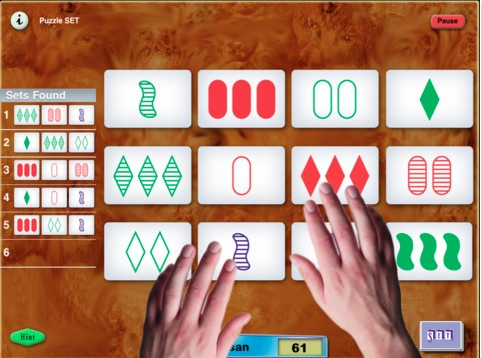
\includegraphics[height=.25\paperwidth]{img/official.jpg} \hspace{.5cm}
 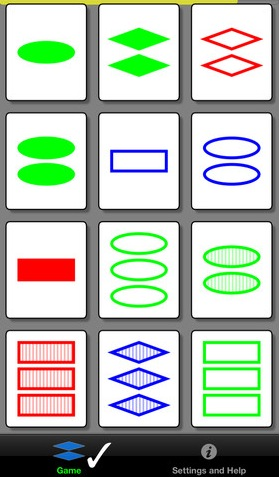
\includegraphics[height=.25\paperwidth]{img/zotz.jpg} \hspace{.5cm}
 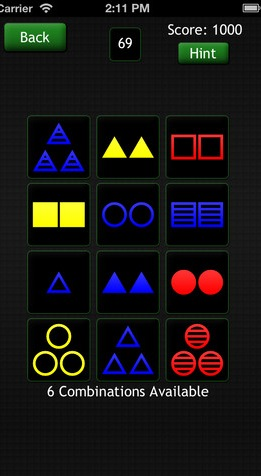
\includegraphics[height=.25\paperwidth]{img/combinations.jpg}
\end{figure}

\end{frame}

\section{Specifications}
\begin{frame}[t]{Game Requirements}
\textbf{Essential:}
\begin{itemize}
 \item Free and functional
 \item Clutter-free gameplay
 \item Control over gameplay
 \item True to the original
\end{itemize}
\pause
\vspace{.5cm}
\textbf{It would be cool if:}
\begin{itemize}
 \item Player statistics
 \item Multiplayer on a single device
 \item Multiplayer on peer-to-peer network
\end{itemize}
\end{frame}

\section{Demo}
\begin{frame}{Demo}
 
\begin{figure}
 \centering
 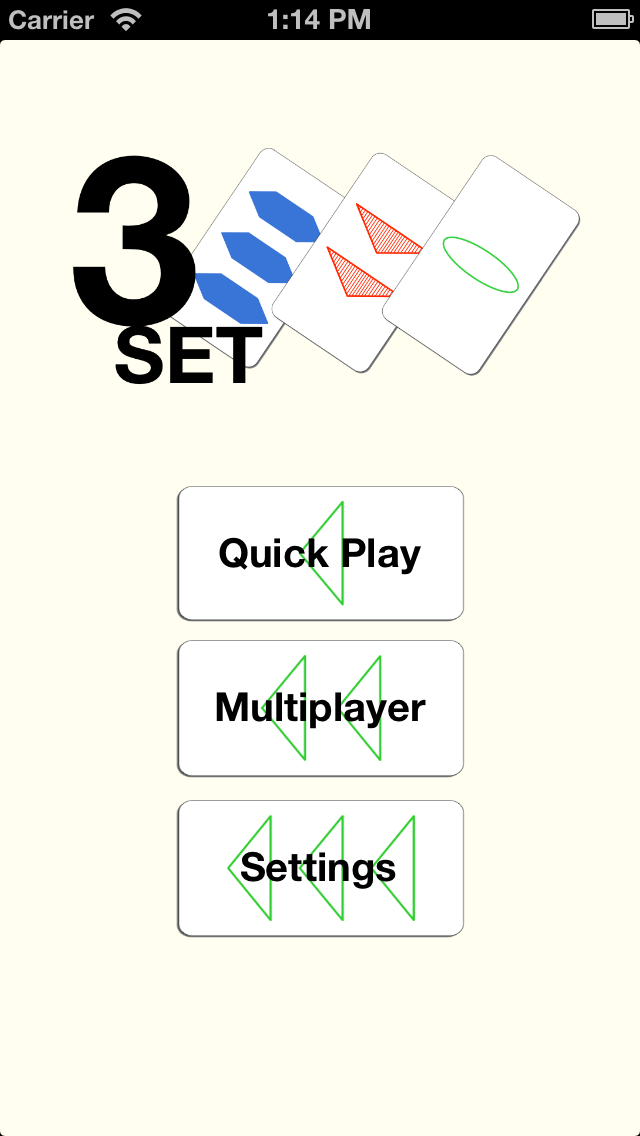
\includegraphics[width=.3\paperwidth]{img/landing.png}
\end{figure}
\end{frame}

\section{Implementation}

\begin{frame}[t]{Back-End Overview}
\textbf{Objective-C}:
\begin{itemize}
 \item View-ViewController-Model Paradigm
 \item Views can be designed with Storyboard editor
\end{itemize}
\pause
\vspace{.5cm}
\textbf{Design Challenges:}
\begin{itemize}
 \item Dynamic grid with resizing, rearranging cards
 \item Managing images efficiently
\end{itemize}

\end{frame}

\begin{frame}[t]{Back-End Overview}

\begin{figure}
\centering
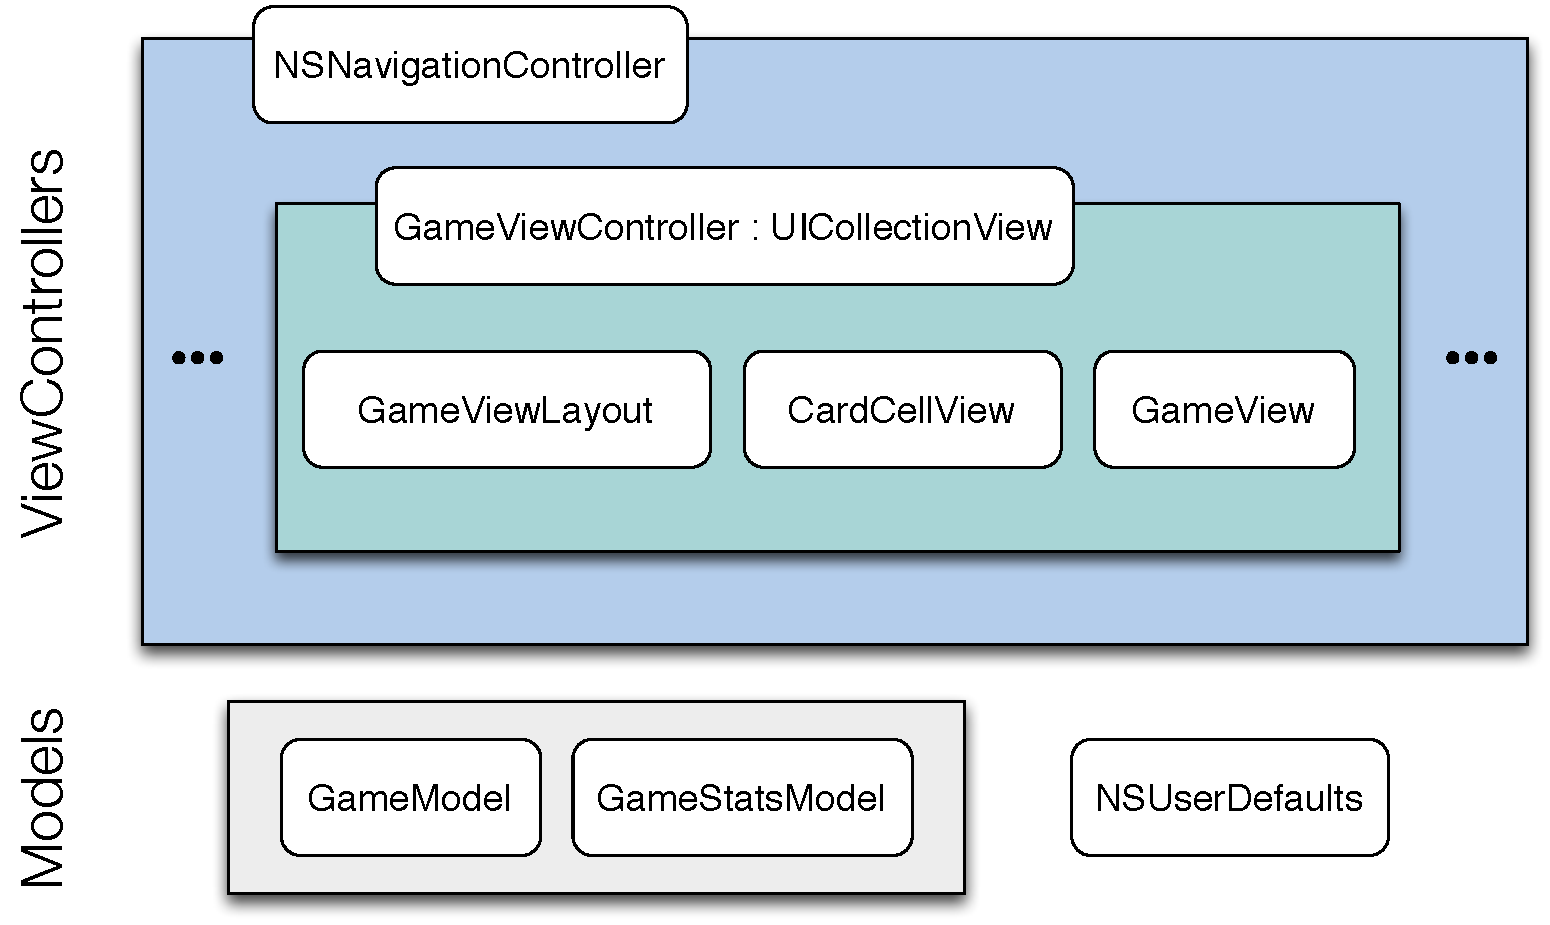
\includegraphics[width=.8\paperwidth]{img/design.pdf} 
\end{figure}
\end{frame}

\section{Future Work}
\begin{frame}[t]{Future Work}
 \textbf{Surface Changes}:
\begin{itemize}
 \item Modify artwork for clarity
 \item Deal-in animations
 \item Additional settings options
\end{itemize}

\pause
\vspace{.5cm}

 \textbf{Additional Features}:
\begin{itemize}
 \item Multiplayer on one device
 \item Game Center integration
 \item Generalized n-Set
\end{itemize}
\end{frame}



\end{document}